\documentclass{article}
\oddsidemargin 0in \evensidemargin 0in \topmargin 0in
\columnsep 10pt \columnseprule 0pt 
\marginparwidth 90pt \marginparsep 11pt \marginparpush 5pt 
\headheight 0pt \headsep 0pt 
%\footheight 0pt \footskip 0pt 
\textheight 9.0in \textwidth 6.5in

\usepackage{graphicx}

\begin{document}
\hspace{2in} Name: \underline{SOLUTION}\\

\begin{center}
{\large STATISTICS 201 - Written Homework Chapter 6}\\[3mm]


\end{center}

\begin{enumerate}
\item {\em (5 pts)} For the Somerset neighborhood 2009 Ames sales data tabulate the correlations between the SalePrice, LotArea, LivingArea and GarageArea. (See the textbook for an example of how to do this. Be sure to round numbers appropriately.)

%\includegraphics[width=5in]{somerset-cor.png}

\begin{tabular}{l|rrrr}
 & SalePrice & LotArea & LivingArea & GarageArea \\\hline
SalePrice & 1.00 & 0.54 & 0.63 & 0.55 \\
LotArea & & 1.00 & 0.31 & 0.62 \\
LivingArea & & & 1.00 & 0.50 \\
\end{tabular}

\begin{enumerate}
\item {\em (2 pts)} Which two variables have the strongest correlation? What is it?

{\em SalePrice and LivingArea}

\item {\em (3 pts)} Make scatterplots of each of the pairs of variables (don't hand these in). Write a paragraph briefly describing the associations, and discussing whether correlation is  or isn't an appropriate summary.

{\em Based on the scatterplots, we can say that generally there is positive association between all of these variables. If the lot area is bigger then so is the living area and garage area, and also the sale price of the home. There are some patterns between some of the variables which would make correlation not the best summary of the association. For example, between sale price and lot area we can see clusters, and within these clusters the association varies a little. There are also some outliers which may affect the correlation, for example, one house that has a sale price close to \$500000, much higher than all of the others in the data set. }

\end{enumerate}

\item Fit a regression model for SalePrice against LivingArea. 

\begin{enumerate}
\item {\em (2 pts)} Write out the model. 

\[
\hat{y} = 68548.0 + 96.9x
\]

\item {\em (2 pts)} Print the scatterplot and sketch the linear model on this plot. 

{\em Predict values for $x=1200$ gives $\hat{y}=184843.7$ and $x=2000$ gives $\hat{y}=262374.1$  respectively. Plot these two points and draw the line between. }

\centerline{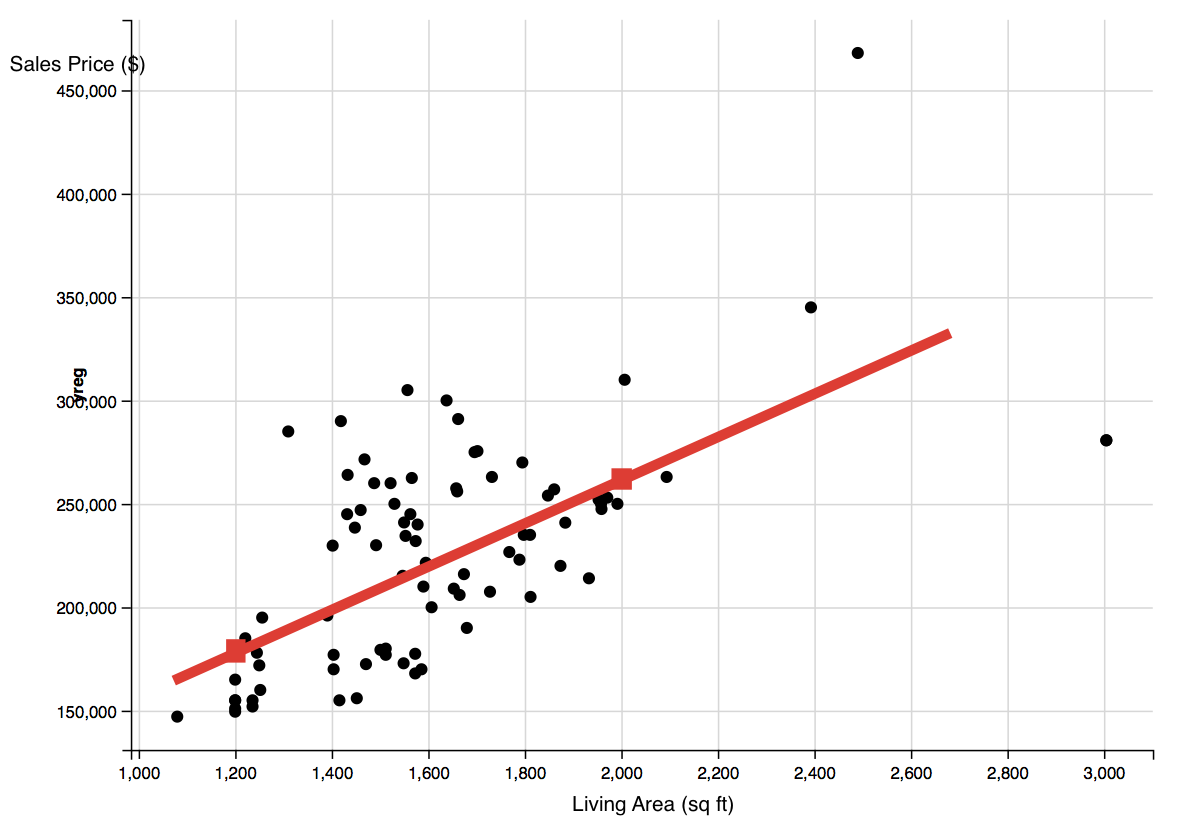
\includegraphics[width=4in]{hmwkch6-7-scatplot.png}}

\item {\em (2 pts)} What proportion of variation in house price does the living area explain?

\[
R^2 = 0.40
\]

\item
{\em (2 pts)} Predict the average sales price for a house having 1500 sq ft of living space.

\[
68548.0 + 96.9\times 1500 = 213917.6
\]

\item {\em (2 pts)} There is a (small) problem with the fit. Diagnose this using the residual plots, and write a paragraph on how you would correct it, and re-fit the model. 

{\em There is a large house (3000 sq ft) that sold for a relatively low price of  approximately \$285,000. It is clear from the residual plot that it pulls the regression line away from the rest of the points, so that the trend is not accurately captured by the model. It would be a good idea to remove this house from the data and re-fit the model, to examine the influence of this point. If the slope and intercept of the model changes by a lot then this house should be considered to have some special qualities which differ from the other houses in the data base, and removed from the analysis.}

\end{enumerate}

\end{enumerate}

\end{document}
